\subsection{The Fetcher: External Clock and Pull model}

The design philosophy of Databus is that it is simply a transporter of changes that have been committed upstream. Each change or change-set is expected to be annotated with a monotonically increasing clock value which we refer to as the SCN of the change or change-set. As changes flow throughout the data architecture, derived state gets created by applications and needs to be associated back to the change stream that generated that state. This is important not just for auditing, but also to recover from failures and resume processing without missing any changes. 
The entire Databus infrastructure therefore tracks the lineage of data records and the progress of consumers using only the clock of the external system. Physical offsets in transport are only used as optimizations but are never used as source of truth. This is a very important design decision because it allows an application to bootstrap itself with a snapshot of data that it might have procured outside the Databus ecosystem. For example, an application can take a dump of an Oracle database, perform arbitrary processing on that dump, and then seamlessly tap into the Databus stream to get all changes that have happened to the database without missing a single change. The only requirement is that the original Oracle dump should be stamped with the same clock that the Oracle Databus fetcher uses to pull changes out from Oracle. Figure~\ref{fig:pull-model} shows the interactions between the different fetcher components and the source clock across the relay, bootstrap log and snapshot store. In this example, the source has generated changes until sequence number 102400, the relay has an in-memory buffer that covers all changes from 70000 to 100000, the bootstrap server's persistent log covers all changes from 30000 to 90000, and the bootstrap server's snapshot store covers all changes from 0 to 80000. Depending on where the consumer is currently at, it will pull from either the relay or the bootstrap server. 

\begin{figure}
\centering
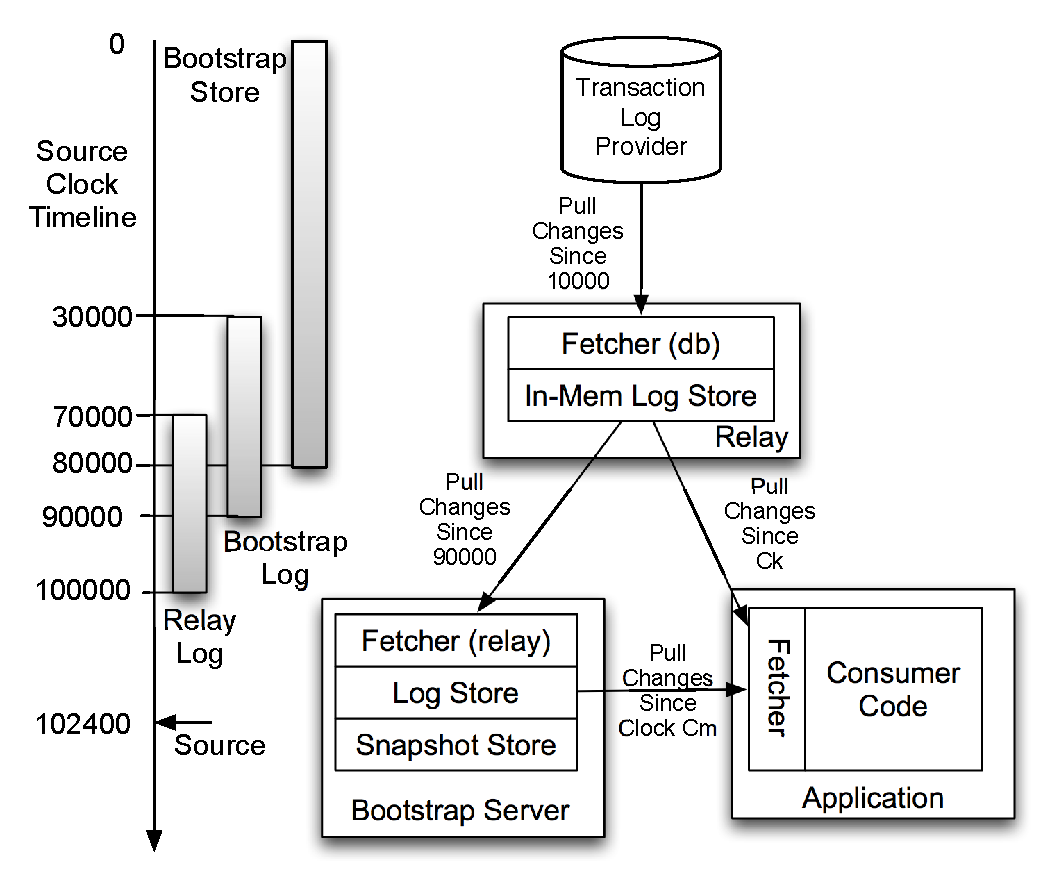
\epsfig{file=figures/databus-pull-model.eps, scale=0.50}
\caption{Pull Model and Source Clock}
\label{fig:pull-model}
\end{figure}

Fetchers keep track of where they are in the timeline using checkpoints which typically contain a highwatermark corresponding to the contiguous section of the timeline that has been reliably processed so far. The fetcher is expected to be initialized with a checkpoint when it starts up or recovers from a failure. Once initialized, the fetcher keeps pulling changes from the data-source from that checkpoint onwards. As changes get processed, the fetcher keeps advancing the highwatermark and periodically stores the checkpoint in some persistence layer. This pure pull model ensures that the Databus transport layer is lossless. The only guarantees needed from the persistence layer is to not lose changes out of order. Similarly, the only requirement this adds on the data source is that it should be able to support rewindable consumption; the fetcher can sometimes go back in time on failures. In most of the systems we've seen, this requirement does not add extra complexity on the source as long as this lookback window is bounded (within a day or two). The way the Oracle fetcher is written, it can go back all the way to time zero, but at the cost of queries that get progressively expensive. The MySQL fetcher can rewind back to as much time as the storage on the MySQL machine will allow to retain, without any performance penalties. This centralization of complexity onto the fetcher component leads to very simple persistence and failure-recovery protocols downstream.
